\documentclass[aspectratio=169]{beamer}

\usepackage[utf8]{inputenc}
\usepackage[T1]{fontenc}
\usepackage{amsmath}
\usepackage{graphicx}
\usepackage{tikz}
\usetikzlibrary{calc}

\usetheme[language=english]{LTU}

% Diagrams (D2, theme 200) live in figures/ ; theme art lives in media/
\graphicspath{{figures/}{media/}}

% A generated diagram, sized to leave room for explanatory text below it.
\newcommand{\diagram}[2][0.5\paperheight]{%
  \begin{center}\includegraphics[height=#1,width=0.92\paperwidth,keepaspectratio]{#2}\end{center}}

% The BuildSim screenshot (its own dark UI, shown larger).
\newcommand{\shot}[1][0.66\paperheight]{%
  \begin{center}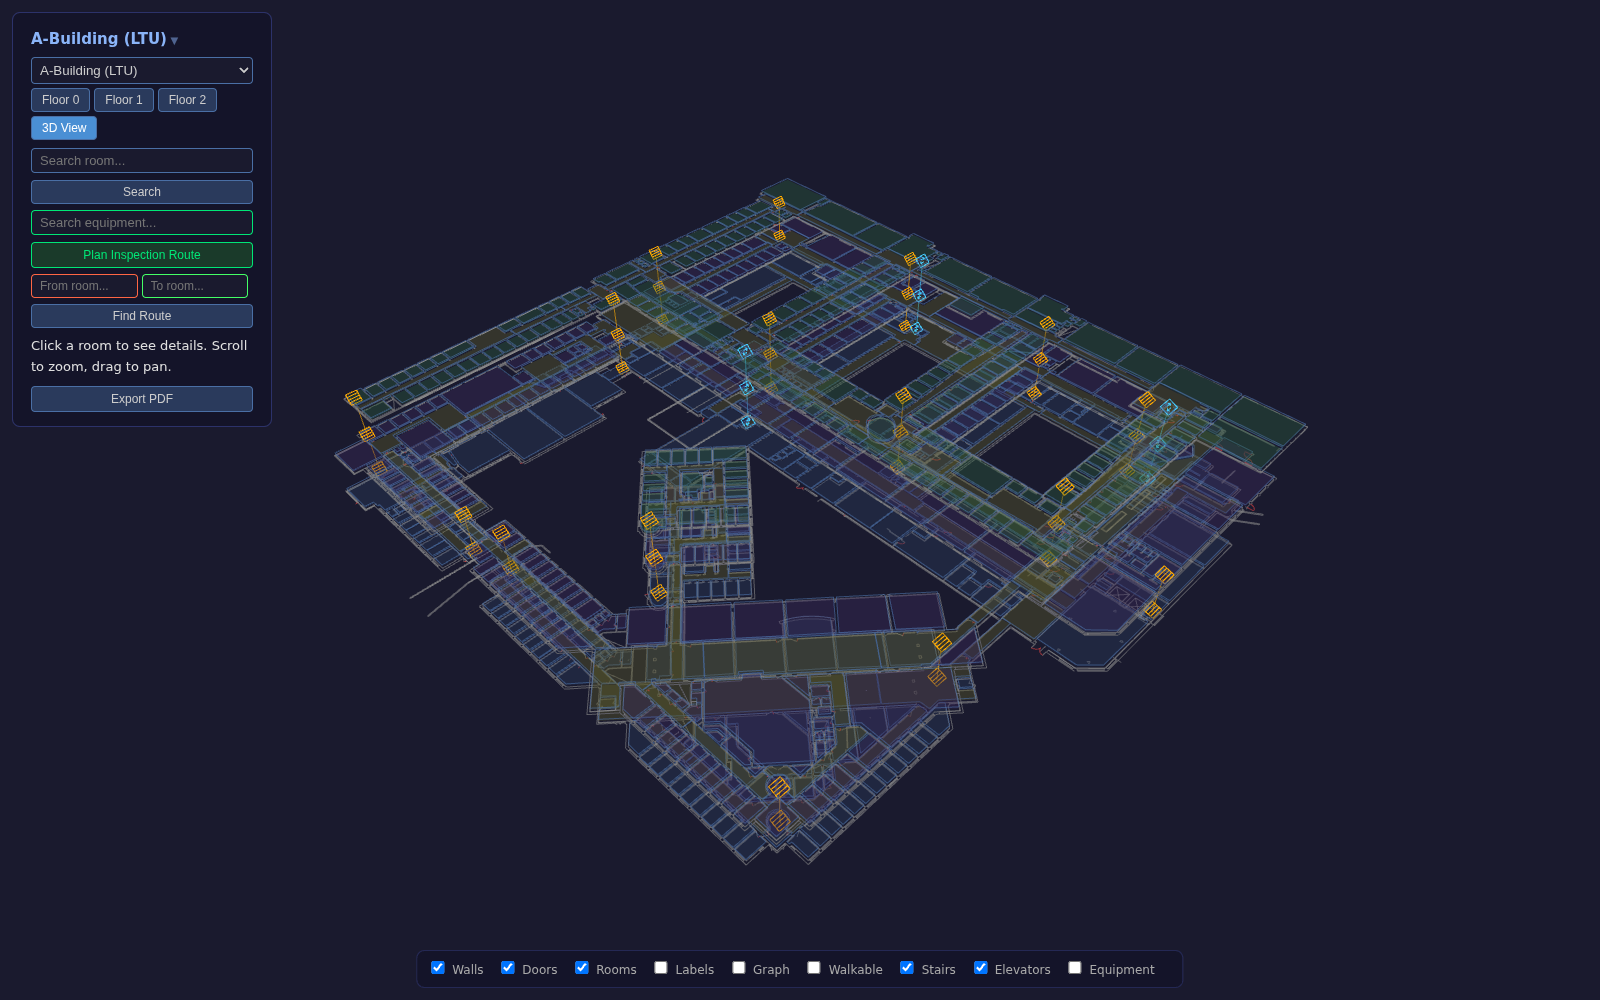
\includegraphics[height=#1,width=0.8\paperwidth,keepaspectratio]{buildsim}\end{center}}

\setbeamertemplate{itemize/enumerate body begin}{\footnotesize}
\newcommand{\expl}[1]{\par\vspace{0.2em}{\footnotesize #1}}

% A simple part-divider frame.
\newcommand{\partframe}[2]{%
  \begin{frame}[plain]
    \begin{tikzpicture}[remember picture, overlay]
      \node at ($(current page.center)+(0,0.06\paperheight)$)
        {\usebeamerfont{frametitle}\color{accentColor}\Huge #1};
      \node at ($(current page.center)+(0,-0.08\paperheight)$)
        {\color{white}\Large #2};
    \end{tikzpicture}
  \end{frame}}

\title{Embedded Intelligence at the Edge}
\subtitle{D7065E}
\date{Lecture 1 \textendash{} Introduction \quad 31 August 2026}
\author{Johan Kristiansson \textbar{} Luleå University of Technology}

\begin{document}

% ---------------------------------------------------------------- Title
\begin{frame}
  \titlepage
\end{frame}

% ---------------------------------------------------------------- Welcome
\begin{frame}{Welcome to D7065E}
  \footnotesize
  This course teaches how to design and build \textbf{autonomous intelligent systems}
  that \textbf{sense, reason, and act} in physical environments, at the intersection of
  \textbf{edge computing}, \textbf{AI agents}, and \textbf{cyber-physical systems (CPS)}.
  \vspace{0.6em}
  \begin{itemize}
    \item \textbf{The project:} instrument a \emph{simulated smart building} with sensors
      and actuators, then build software that makes real-time control decisions.
    \item \textbf{Open-ended:} teams choose the control problem, architecture, communication
      patterns, and autonomous approach. There is no single correct solution.
    \item \textbf{A systems engineering course:} the focus is architecture, communication,
      data pipelines, testing, and integration, not advanced AI research.
  \end{itemize}
\end{frame}

% ---------------------------------------------------------------- Roadmap
\begin{frame}{Today}
  \footnotesize
  \begin{columns}[t]
    \begin{column}{0.33\textwidth}
      {\color{accentColor}\normalsize Part A}\\[0.2em]
      \textbf{The course.}\\ How it runs, what you deliver, how it is graded and examined.
    \end{column}
    \begin{column}{0.33\textwidth}
      {\color{accentColor}\normalsize Part B}\\[0.2em]
      \textbf{The field.}\\ An introduction to cyber-physical systems, the edge, and autonomy.
    \end{column}
    \begin{column}{0.33\textwidth}
      {\color{accentColor}\normalsize Part C}\\[0.2em]
      \textbf{The system.}\\ BuildSim, the architecture, and what you build.
    \end{column}
  \end{columns}
\end{frame}

% ================================================================ PART A
\partframe{Part A}{The course}

\begin{frame}{What you will learn}
  \footnotesize
  \begin{itemize}
    \item Design \textbf{CPS architectures} connecting sensors, computation, and actuators into autonomous control loops.
    \item Apply \textbf{model-based, specification-driven} methods to design, implement, and validate systems.
    \item Build \textbf{data pipelines} that collect, store, and transform sensor data for decision-making.
    \item Develop \textbf{autonomous services and agents} that observe state, reason, and act.
    \item Evaluate \textbf{resilience, safety, scalability, and performance} under failures and uncertainty.
  \end{itemize}
\end{frame}

\begin{frame}{How the course runs}
  \footnotesize
  \begin{enumerate}
    \item Choose a use case (or propose your own).
    \item Write an \textbf{architecture document} and design specification.
    \item Write a \textbf{test plan}.
    \item Get the design \textbf{approved} at the week-3 checkpoint.
    \item Implement the system.
    \item Demonstrate and defend your results.
  \end{enumerate}
  \expl{The architecture document is a \textbf{living document}: start it once the proposal is approved,
  and refine it as the system is built.}
\end{frame}

\begin{frame}{What you deliver}
  \diagram[0.44\paperheight]{deliverables}
  \footnotesize An \textbf{architecture document} (C4 context + container, requirements table,
  interface contracts), a \textbf{test plan} with results, the \textbf{running system + dashboard},
  a \textbf{written report}, the \textbf{source code} in git, and an \textbf{individual oral defence}.
\end{frame}

\begin{frame}{Three kinds of thinking}
  \diagram[0.46\paperheight]{thinking}
  \footnotesize The course develops \textbf{architectural}, \textbf{systems}, and \textbf{critical}
  thinking. Your grade reflects these skills, not the number of features or the sophistication of the
  AI. A simple system that is well-designed, well-justified, and critically evaluated scores higher
  than a complex one that cannot be explained.
\end{frame}

\begin{frame}{How it is graded}
  \diagram[0.42\paperheight]{grading}
  \footnotesize \textbf{Stage 1} is a Pass/Fail gate of mandatory requirements, miss one and the
  project is \textbf{U} until fixed. \textbf{Stage 2} grades four dimensions (A\textendash D) at levels
  \textbf{3/4/5}, judged \emph{holistically}: a serious weakness in one dimension limits the grade.
\end{frame}

\begin{frame}{The four graded dimensions}
  \footnotesize
  \begin{itemize}
    \item \textbf{A. Architecture \& design} \textemdash{} documented, justified, evaluated (LO2).
    \item \textbf{B. Systems integration \& the CPS loop} \textemdash{} the whole loop, failure
      behaviour, emergent effects (LO1, LO3).
    \item \textbf{C. Autonomous services \& data engineering} \textemdash{} decisions backed by a
      data pipeline, data-quality handling (LO1, LO3).
    \item \textbf{D. Critical evaluation} \textemdash{} testing, fault injection, stress and
      breaking-point analysis, honest critique (LO4).
  \end{itemize}
\end{frame}

\begin{frame}{Expectations and scope}
  \footnotesize
  \begin{itemize}
    \item This is a \textbf{systems engineering} course: architecture, communication, pipelines,
      testing, and integration come first.
    \item Apply core \textbf{distributed-systems} concepts: decomposition, APIs, messaging,
      containers, fault handling.
    \item You are \emph{not} expected to implement consensus protocols, distributed databases, or
      large-scale cloud infrastructure, those come in later courses.
    \item \textbf{Simple, well-done beats complex and unexplained.} More AI does not mean a higher grade.
  \end{itemize}
\end{frame}

\begin{frame}{Examination}
  \footnotesize
  \begin{itemize}
    \item The project is done \textbf{in pairs}; it is open-ended, with no single correct answer.
    \item Each student takes an \textbf{individual oral exam} ($\sim$30 min): a 10-minute live demo,
      then a 20-minute \textbf{whiteboard} session, \emph{no slides or notes}.
    \item The oral is a \textbf{gate, not a modifier}: it cannot raise the project grade, only confirm
      the level each student can \emph{personally} explain and defend.
    \item Teammates may receive \textbf{different grades}. Cannot defend your own system $\Rightarrow$ U.
  \end{itemize}
\end{frame}

\begin{frame}{The oral exam: what you must be able to do}
  \footnotesize
  Draw and explain, from memory: the \textbf{architecture} and component responsibilities; how the
  system \textbf{senses, reasons, and acts}; how \textbf{data flows} from sensing to action; and your
  \textbf{testing} and failure behaviour.
  \vspace{0.4em}

  Be ready for questions such as:
  \begin{itemize}
    \item What makes a system \emph{autonomous} rather than \emph{automated}?
    \item What happens if a sensor lies, or a decision component becomes unavailable?
    \item Why this communication pattern? What are the main failure modes? How would it scale?
  \end{itemize}
\end{frame}

\begin{frame}{AI-assisted development}
  \footnotesize
  Agentic coding tools (Claude Code, Codex, Cursor, Cline, Aider) can autonomously read code, edit
  files, run commands, and write tests, and are \textbf{strongly encouraged}; they can dramatically
  increase development speed and project scope.
  \vspace{0.5em}
  \begin{itemize}
    \item You remain \textbf{responsible} for every design decision, line of code, test, and conclusion.
    \item The oral exam assesses \textbf{your} understanding, not the AI's ability to generate the system.
  \end{itemize}
\end{frame}

\begin{frame}{Lectures and deadlines}
  \diagram[0.4\paperheight]{timeline}
  \footnotesize Lecture 1 (today): introduction. \textbf{Sep 2}: form lab groups. \textbf{Sep 4}:
  BuildSim workshop. \textbf{Sep 11}: submit the proposal. Design approved by week 3, then build.
  \textbf{Oct 12}: final submission. \textbf{Oct 14\textendash19}: demonstration and oral examination.
\end{frame}

% ================================================================ PART B
\partframe{Part B}{Cyber-physical systems, edge computing, and autonomy}

\begin{frame}{What is a cyber-physical system?}
  \diagram[0.42\paperheight]{cps-generic}
  \footnotesize A \textbf{cyber-physical system (CPS)} tightly integrates computation, networking, and
  physical processes [1,2]. It runs a continuous
  \textbf{sense $\rightarrow$ compute $\rightarrow$ act} loop: the \emph{cyber} part senses only through
  sensors and acts only through actuators; the \emph{physical} part evolves by physics and human
  behaviour, and never stops, even when no computer is watching.
\end{frame}

\begin{frame}{Cyber-physical systems are everywhere}
  \diagram[0.5\paperheight]{cps-examples}
  \footnotesize Described as the \emph{next computing revolution} [2], CPS underpin
  cars, factories, energy grids, and buildings: \textbf{sensors $\rightarrow$ control $\rightarrow$
  actuators} in a continuous loop. This course uses a \emph{building} as its cyber-physical system.
\end{frame}

\begin{frame}{From cloud to edge}
  \footnotesize
  As billions of sensors came online, sending every reading to a distant data centre became too slow,
  too costly in bandwidth, and a single point of failure.
  \begin{itemize}
    \item \textbf{Fog computing} [5] introduced a layer between devices and the cloud
      to support latency-sensitive, geographically distributed applications.
    \item \textbf{Edge computing} [3,4] pushes computation to the edge of the
      network, \emph{next to the data sources}, rather than into the cloud.
  \end{itemize}
  \expl{The shift is driven by latency, bandwidth, reliability, and privacy, the recurring themes of
  \emph{edge intelligence}.}
\end{frame}

\begin{frame}{Edge computing: bring computation to the data}
  \diagram[0.44\paperheight]{edge-vs-cloud}
  \footnotesize \textbf{Edge} computing places computation next to the sensors: millisecond latency,
  and it keeps working when the network does not [3,4]. The \textbf{cloud}
  is far away and depends on connectivity. A real-time control loop belongs at the edge.
\end{frame}

\begin{frame}{The edge-cloud continuum}
  \diagram[0.44\paperheight]{continuum}
  \footnotesize Computation is not edge \emph{or} cloud but a \textbf{continuum}: fast inference near
  the sensors, heavier training pushed out to a local server or the cloud/HPC, with updated models
  flowing back. Managing resources and placement across this continuum is Learning Outcome~1.
\end{frame}

\begin{frame}{Data engineering for CPS}
  \diagram[0.42\paperheight]{data-eng}
  \footnotesize Sensor data arrives with \textbf{volume, velocity, and variety}. It is ingested
  (stream or batch), refined through a \textbf{data lake}, raw $\rightarrow$ cleaned $\rightarrow$
  feature, the \emph{medallion} pattern, and served from a \textbf{time-series database} for live
  queries, turning raw readings into features an autonomous component can use.
\end{frame}

\begin{frame}{From automation to autonomy}
  \diagram[0.46\paperheight]{agent-loop}
  \footnotesize Automation comes in three generations: \textbf{rules} $\rightarrow$ \textbf{machine
  learning} $\rightarrow$ \textbf{agentic AI} [8]. An autonomous agent closes a loop,
  \textbf{perceive $\rightarrow$ reason $\rightarrow$ plan $\rightarrow$ act $\rightarrow$ observe},
  using tools to act, with \textbf{guardrails} and human-in-the-loop for safety.
\end{frame}

\begin{frame}{Why the edge matters}
  \footnotesize
  \begin{itemize}
    \item \textbf{Latency} \textemdash{} physical processes cannot wait for a round trip to a data centre.
    \item \textbf{Resilience} \textemdash{} the system keeps working when connectivity is lost.
    \item \textbf{Bandwidth} \textemdash{} raw sensor streams are too large to ship everywhere.
    \item \textbf{Privacy} \textemdash{} data can be processed locally instead of leaving the building.
    \item \textbf{Autonomy} \textemdash{} local decisions enable real-time, self-governing behaviour.
  \end{itemize}
\end{frame}

% ================================================================ PART C
\partframe{Part C}{The system you will build}

\begin{frame}{BuildSim: the building, provided for you}
  \shot
  \expl{\textbf{BuildSim} is a single Go binary that bundles a 3D building model, a REST API, and a
  live web viewer. It holds the building state, you build everything around it: the physics, the
  sensors and actuators, the autonomous agent, the data pipeline, and the dashboard.}
\end{frame}

\begin{frame}{BuildSim is the shared state}
  \diagram{system-overview}
  \footnotesize Every component runs as its own process and talks to BuildSim over REST: the
  \textbf{simulator} drives sensor values, the \textbf{agent} reads them and commands \textbf{actuators},
  the \textbf{pipeline} stores the stream, and the browser shows the live 3D view.
\end{frame}

\begin{frame}{A closed feedback loop}
  \diagram{feedback-loop}
  \footnotesize The simulator turns actuator states into the \emph{next} sensor readings, and the
  agent turns readings into commands. \textbf{Actuator commands must change future sensor readings};
  otherwise the loop is open and the control does nothing. This loop is the heart of the project.
\end{frame}

\begin{frame}{Every component is its own process}
  \diagram{processes}
  \footnotesize Sensors, actuators, agent, broker, storage, and dashboard each run as a
  \textbf{separate, containerised} service (e.g.\ \texttt{docker compose}) alongside BuildSim.
  Any process can crash, restart, and re-register. The system must \emph{not} be a single monolith.
  An optional GPU server can host an LLM.
\end{frame}

\begin{frame}{Why a simulated building?}
  \footnotesize
  Testing autonomous control on a real building would be \textbf{slow, costly, unsafe, and hard to
  reproduce}. Instead the project uses \textbf{system-level simulation}: the environment, sensors,
  actuators, communication, and control software are developed and evaluated as one complete CPS.
  \vspace{0.5em}
  \begin{itemize}
    \item Model the building \emph{realistically enough} that the architecture would be unchanged on a
      real building, the goal is not to generate artificial data.
    \item Test, validate, and iterate under controlled, repeatable conditions.
  \end{itemize}
\end{frame}

\begin{frame}{Specification-first, with MBSE}
  \diagram[0.42\paperheight]{mbse}
  \footnotesize Model before code: C4 diagrams, sequence and data-flow diagrams, and requirements
  [6,7]. The models are the \textbf{input to AI tools}, and tests derive
  from the spec. Use \textbf{lightweight artefacts}, not SysML, the value is the engineering thinking, not the notation.
\end{frame}

\begin{frame}{Pick a use case}
  \diagram[0.46\paperheight]{usecases}
  \footnotesize Choose one or \textbf{propose your own} (subject to approval). Every project needs
  sensors, a data pipeline, autonomous decisions, and a dashboard, and must include a
  \textbf{data-driven component} (ML, anomaly detection, forecasting, optimisation), not just fixed
  thresholds.
\end{frame}

\begin{frame}{What you must build (Pass/Fail requirements)}
  \footnotesize
  \begin{itemize}
    \item Sensor, actuator, and decision components run as \textbf{separate, restartable processes}.
    \item The system works \textbf{end-to-end}: sensing $\rightarrow$ decision $\rightarrow$ actuation
      $\rightarrow$ a visible effect in BuildSim that feeds back into the next readings.
    \item At least one component performs \textbf{autonomous decision-making} from sensor data.
    \item A \textbf{data pipeline} collects, stores, and serves sensor data.
    \item An \textbf{architecture document}: C4 context + container diagrams, requirements table, interfaces.
    \item A \textbf{test plan}, executed: unit tests, $\geq 1$ end-to-end test, documented results.
    \item A \textbf{dashboard}, a \textbf{written report}, and an oral defence \emph{from memory}.
  \end{itemize}
  \expl{Missing any one of these means \textbf{U (Fail)} until it is addressed.}
\end{frame}

\begin{frame}{The physical simulator}
  \footnotesize
  Build a simulator that models your use case and produces \textbf{realistic sensor data that
  responds to actuator commands}, closing the feedback loop. Examples:
  \begin{itemize}
    \item \textbf{Fire:} smoke rises and spreads to adjacent rooms; sprinklers reduce it.
    \item \textbf{HVAC:} temperature depends on outdoor temp, occupancy (body heat), and HVAC state.
    \item \textbf{Air quality:} CO\textsubscript{2} rises $\sim$40\,ppm/person/hour, falls with ventilation.
  \end{itemize}
  \expl{It need not be physically perfect. Capture trends, correlations, and responses to actuators,
  then spend your time on \textbf{architecture, integration, and testing}.}
\end{frame}

\begin{frame}{Occupancy patterns}
  \footnotesize
  Occupancy drives temperature, CO\textsubscript{2}, lighting, and access, so model it realistically:
  \begin{itemize}
    \item Weekdays: arrive 7\textendash9, lunch 11:30\textendash13:00, leave 16\textendash18; weekends empty.
    \item Meeting rooms booked in blocks; corridors briefly occupied in transit.
  \end{itemize}
  \expl{Approaches: physics-based equations, replay of public datasets, a hybrid (real data + injected
  events), or a generative model. Datasets such as ASHRAE, Building Data Genome, and occupancy-detection
  sets are available.}
\end{frame}

\begin{frame}{Data engineering}
  \diagram[0.42\paperheight]{pipeline}
  \footnotesize Sensor data must flow through a \textbf{real pipeline}, not ad-hoc REST calls. Choose
  and justify a \textbf{broker} (MQTT, Kafka, Redis), a \textbf{store} (InfluxDB, TimescaleDB, DuckDB,
  Parquet), and a \textbf{feature pipeline}. Integration options: Arrowhead/SOA, ColonyOS for edge-cloud orchestration.
\end{frame}

\begin{frame}{The autonomous component}
  \footnotesize
  \begin{itemize}
    \item At least one component makes \textbf{autonomous decisions} from sensor data and drives an actuator.
    \item \textbf{Rule-based, optimisation, ML, or LLM} approaches are all acceptable, if genuine,
      justified, and integrated. A \textbf{data-driven} element is required.
    \item It can reason about \emph{sensor data} (anomaly detection, prediction), \emph{text}
      (regulations, manuals), or \emph{both} (an LLM checking readings against rules).
  \end{itemize}
  \expl{\textbf{More sophisticated AI does not mean a higher grade.} The AI is one part of the system.}
\end{frame}

\begin{frame}{Implementation}
  \footnotesize
  \begin{itemize}
    \item Each sensor and actuator is its \textbf{own process}, preferably a Docker container,
      independently startable, stoppable, and restartable.
    \item \textbf{Go} is recommended (single static binaries, strong concurrency, BuildSim is Go).
      Other languages may be used if strongly motivated.
    \item Everything runs \textbf{locally} on the laptop: \texttt{./buildsim start} plus
      \texttt{docker compose up}.
  \end{itemize}
\end{frame}

% ---------------------------------------------------------------- References
\begin{frame}{References and further reading}
  \footnotesize
  \begin{enumerate}
    \item E. A. Lee. Cyber Physical Systems: Design Challenges. \emph{IEEE ISORC}, 2008.
    \item R. Rajkumar, I. Lee, L. Sha, J. Stankovic. Cyber-Physical Systems: The Next
      Computing Revolution. \emph{DAC}, 2010.
    \item W. Shi, J. Cao, Q. Zhang, Y. Li, L. Xu. Edge Computing: Vision and Challenges.
      \emph{IEEE Internet of Things J.}, 2016.
    \item M. Satyanarayanan. The Emergence of Edge Computing. \emph{Computer}, 2017.
    \item F. Bonomi, R. Milito, J. Zhu, S. Addepalli. Fog Computing and Its Role in the
      Internet of Things. \emph{MCC Workshop}, 2012.
    \item J. A. Estefan. Survey of Model-Based Systems Engineering (MBSE) Methodologies.
      \emph{INCOSE}, 2007.
    \item S. Brown. Software Architecture for Developers, Vol.~2, the C4 model. 2018.
    \item S. Russell, P. Norvig. Artificial Intelligence: A Modern Approach. 4th ed., 2021.
  \end{enumerate}
  \vspace{0.3em}
  Syllabus: \texttt{ltu.se/.../course-syllabus?id=D7065E} \,\textbullet\,
  C4 model: \texttt{c4model.com} \,\textbullet\,
  BuildSim: \texttt{buildingsim/docs/lab-quickstart.md}
\end{frame}

\end{document}
